\documentclass[12pt,letterpaper,ngerman]{article}
%\usepackage[letterpaper,top=3.0cm, bottom=3.0cm, footnotesep=1.0cm]{geometry}
\usepackage[letterpaper,margin=1in]{geometry} % e. Set margins of 1 inch (2.54 cm.) on all four sides of the paper. 
\usepackage{mathptmx} % d. ...in a simple roman face except where indicated below (§3). 
\usepackage[singlespacing]{setspace} % Set line spacing to 1 throughout the document
\usepackage{fancyhdr} 

% Set the headheight to at least 14.49998pt
\setlength{\headheight}{14.49998pt}

% Optionally adjust \topmargin if necessary
% \addtolength{\topmargin}{-2.49998pt}
\usepackage{relsize}

\usepackage[bottom]{footmisc}
\usepackage{tabularx}
    
\pagestyle{empty}        % No page numbers

% Set paragraph indentation to 1.5cm
\setlength{\parindent}{2em}

%%%Using XeTeX (xelatex, lulatex):
%\usepackage{polyglossia}
%\usepackage{fontspec}
%\usepackage{xunicode}
%\usepackage{xltxtra}
\usepackage{url}
\usepackage{hyperref}
\usepackage[english,german]{babel}

\usepackage{graphicx}

%\setmainfont[Mapping=tex-text]{Linux Libertine O} %Falls nicht vorhanden müssen die LinLibertine-ttf-Dateien nach C:\windows\fonts verschoben werden

\usepackage{booktabs}    % For nice-looking tables
\usepackage{natbib}      % Citation support (required for crossrefs)
\usepackage{expex}
\bibpunct[:]{(}{)}{;}{a}{}{,} % Defaults for in-text citations
\usepackage{bibentry}    % Print individual references

\usepackage{acronym}
\usepackage{multicol}

% TODO: set authors name
%vorgelegt von\\
%Name des Verfassers/der Verfasserin\\
\author{Author's name}

\usepackage{scrhack} % Recommended to avoid potential conflicts
\usepackage{microtype}

\usepackage[acronym,xindy,toc]{glossaries} % TODO: include "acronym" if glossary and acronym should be separated
\makeglossaries
\loadglsentries{pages/glossary.tex} % important update for glossaries, before document

\usepackage{ragged2e}

% Set up hyphenation rules for the language package when mistakes happen
\babelhyphenation[english]{
an-oth-er
ex-am-ple
}

\usepackage{babel}
\usepackage{csquotes}
\MakeOuterQuote{"}
\usepackage{mathtools}
\usepackage{amssymb}
\usepackage{amsmath}
\usepackage{tikz}
\usepackage{chngcntr}
\usepackage{float}
\usepackage{svg}
\usetikzlibrary{
  decorations.pathmorphing,
  automata, positioning, arrows, matrix,
  decorations.pathreplacing,
  shapes.geometric, calc,shapes.misc,
  arrows.meta,backgrounds,fit,petri
}
\pgfmathsetseed{\number\pdfrandomseed} % to ensure that it is randomized
\begin{document}
\DeclarePairedDelimiter\ceil{\lceil}{\rceil}
\DeclarePairedDelimiter\floor{\lfloor}{\rfloor}
\newcommand{\rand}[2]{
\pgfmathsetmacro{\thenum}{rand(0,1)}
\thenum
}
\newcommand{\nat}[0]{\mathbf{N}}
\newtheorem{example}{Beispiel}[section]


\begin{center}\uppercase{Ludwig-Maximilians-Universität München}\end{center}
\begin{center}
  \uppercase{Programming languages and artificial intelligence}
\end{center}

\vspace*{10mm}
\begin{center}

\includegraphics[height=40mm]{abb/sigillum.png}
\end{center}
\vspace*{10mm}

\title{Titel der Arbeit}
\date{\vspace{-5ex}}
{\let\newpage\relax\maketitle}
\thispagestyle{empty}
\begin{center}
\begin{large}
\begin{Large}
Bachelorarbeit\\
\end{Large}
im Studiengang 'Informatik plus Mathematik' \\
\end{large}
\end{center}
\vspace{1cm}
\begin{center}
\begin{large}
Betreuer: Prof. Dr. Johannes Kinder\\
\end{large}
\end{center}
\begin{center}
\begin{large}
Mentor: Moritz Dannehl, M.Sc.\\
\end{large}
\end{center}


\begin{center}
\begin{large}
Ablieferungstermin: \date{\today} \\
\end{large}
\end{center}

\vspace{1,5cm}

\newpage
\tableofcontents
\newpage

\setcounter{page}{1}
\pagestyle{fancy}
\fancyhf{}
\counterwithin{figure}{section}
\fancyhead[R]{\thepage}
\renewcommand{\headrulewidth}{0pt} %obere Trennlinie
\newtheorem{definition}{Definition}
\section*{Abstract}
\section{Einführung}
In den letzten Jahren gab es große Fortschritte in der natürlichen
Sprachverarbeitung, besonders hervorzuheben sind Large Language Models
die sich mittlerweile in vielen Bereichen der Informatik in die Lösungsansätze
für Problemen in jeweiligen Bereichen eingeschlichen haben. Diese Arbeit
untersucht nun, ob diese Fortschritte in der natürlichen Sprachverarbeitung
eine Hilfestellung leisten können um Source Code Funktionen semantisch sinvoll
in einen Vektor mit reelwertigen Zahlen zu codieren. Diese Vektoren können dann
später als Label verwendet werden um ein Modell zu trainieren was Binary Code 
als Input nimmt und diesen ebenfalls in einen semantischen Vektor mit reelwertigen
Zahlen codiert. Das resultierende Modell kann hinterher verwendet werden um Reverse 
Engeneering zu erleichtern. Ein einfaches Beispiel ist folgendes: Man stelle
sich vor, dass man eine Funktion die in Binary Code vorliegt, mühsehlig manuell
verstanden was für eine Aufgabe die Funktion in der Code Base hat. Nun kann man
diese Funktion codieren und über die Gesamte Code Base einen Nearest Neighbor
Search durchführen und all ähnlichen Funktionen ausgeben lassen.
Das spart zeit, denn nun hat man eine Idee was diese anderen
Funktionen für eine Aufgabe in der Code Base erfüllen könnten.\\
Das oben berschriebene Problem Source Code Vektoren in sinvoll semantische 
reelwertige Vektoren zu codieren ist sehr ähnlich zu einen Problem 
in der natürlichen Sprachverarbeitung und dort bereits gelöst. Die rede ist
von dem Problem einen gegebenen Satz in einen semantisch sinvollen Vektor
abzubilden. Es ist nageliegend zu versuchen dieses Ergebnis der natürlichen
Sprachverarbeitung zu benuzten um eine Lösung für unser Problem zu konstruieren.
Die intuivste Idee ist es einfach die Funktionsnamen, die in natürlicher Sprache
verfasst sind als beschreibung der Funktion zu verwenden. Diese Beschreibunf können
wir nun mühelos codieren, da sie in natürlicher Sprache vorliegt.
Eine zweite Idee ist, die Kommentare der Funktionen, die in natürlicher Sprache
verfasst sind, als Beschreibung der Funktion zu verwenden. Am viel versprechsten
ist es die Funktionen von einen Large Language Modell in natürlicher Sprache
beschreiben zu lassen. Als letztes habe ich noch ein bestehendes Modell
Code2Vec verwendet und es für dieses Problem angepasst.
\pagebreak
\section{Grundlagen und Termini}
\subsection{Maschienelles Lernen}
Heutzutage ist maschienelles Lernen weitverbreitet und wird in nahezu jeden
Bereich der Informatik verwendet.
In diesen Abschnitt wird zunächst maschinelles lernen definiert und 
dann darauf aufbauend grundlegende Trainingsarten vorgestellt.
Maschinelles Lernen wird überall dort eingesetzt
wo eine anayltische Lösung eines Problems zu aufwendig oder gar überhaupt nicht
existiert. % Book: Learingin from data, page 1, row 6
Diese Lösung durch maschinelles Lernen versucht aus den Daten ein Muster
abzuleiten. Bei einer endlichen Menge an Daten ist meist,
das resultierende Modell nur eine Approximation der gesuchten Lösung.
\subsubsection{Definition}
Trotz des bekanntheitsgrades, gibt es den irreglauben, dass
maschinelles lernen nur was mit Neuronalen Netzwerken zu tun
hat, diese Anahme ist im allgemeinen falsch. Generell kann
ein Problem das mit maschinelles Lernen gelöst wird, wie folgt 
formulliert werden:
\begin{definition}
  Sei $X$ eine beliebige Input Menge, $Y$ eine beliebige Output Menge,
  $f \in \{X \to Y\}$ die gesuchte Lösung des Problems, 
  $\mathbb{D}$ eine beliebige Menge aus gegebenen Datenpunkten,\\
  $H_1 \subset \{X \to Y\}$ ein Hypothesenraum, und 
  $A_1: \mathcal{P}(\{X \to Y\}) \times 
  \mathcal{P}(\mathbb{D}) \to \{ X \to Y \} $
  ein Lernalgorithmus. Dann ist das ziel, bei gegebenen Daten,
  den Hypothesenraum $H_1$ und den Lernalgorithmus $A_1$ so zu wählen,
  sodass
  \[
    A_1(H_1, \mathbb{D}) \approx f.
  \]
\end{definition}
Maschinelles lernen ist also die suche nach einen Lernalgorithmus und 
Hypothesenraum, die dann in kombination mit gegebenen Daten, die optimale
Lösung approximieren. Dabei ist hervorzuheben das der Datensatz das Herzstück
jeder Problemstellung im Bereich des maschinellen Lernens ist. Ist der 
Datensatz zu klein oder überhaupt nicht representativ für das gegebene
Probelm, wird der Lernalgorithmus die falschen Muster erkennen und dadurch
eine fehlerhafte Approximation produzieren. % visualisierung.
\begin{figure}[H]
  \begin{center}
    \begin{tikzpicture}
    [inner sep=2mm,
     place/.style={circle,draw=blue!50,fill=blue!20,thick},
     transition/.style={rectangle,draw=black!50,fill=black!20,thick}]
    \node (F) at (-1,4) [transition] {Lösung  $f: X \to Y$};
    \node (D) at (-1,2) [transition] {Datenpunkte $\mathbb{D}$};
    \node (H) at (-1,0) [transition] {Hypothesenraum $H_1$};
    \node (A) at (3,1) [place, label=Lernalgortihmus] {$A_1$};
    \node (FH) at (6,1) [transition, label=Approximation] {$g \approx f$};
    \draw [->] (H) .. controls +(up:8mm) and +(left:8mm)
                         .. (A)
               (D) .. controls +(down:8mm) and +(left:8mm)
                         .. (A);
    \draw[->] (A) -- (FH);
      \draw [->,decorate,
       decoration={snake,amplitude=.4mm,segment length=2mm,post length=1mm}]
      (F) -- (D);
    \end{tikzpicture}
    \caption{Grundlegendes maschinelles Lernen Problem}
  \end{center}
\end{figure}
\hfill
\\
In der Figur 2.1 ist die Problembeschreibung nochmal bildlich dargestellt,
erwähnenswert ist, dass die Datenpunkte nicht immer in abhängigkeit mit $f: X \to Y$
stehen. Beispielsweise können die Datenpunkte einfach nur aus den Eingabewerten
bestehen: $\mathbb{D} = \{x_1,x_2,x_2, \dots, x_n\} \subset X$. Die Struktur
des Datensatzes kann sehr unterschiedlich sein, dass hängt auch mit 
unterschiedlichen Lernmehthoden zusammen.
\subsubsection{Deep-Learning}
Bevor die Lernmethoden genauer betrachtet werden, wird kurz Deep-Learning
vorgestellt. Deep-Learning ist ein Neuronales Netzwerk mit mehreren 
Layern zwischen Input und Output Layer. Zunächst müssen wir jedoch
Neuronale Netzwerke definieren. 
\begin{definition}
  Ein Neuronales Netzwerk (NN) ist eine Funtion $N: \mathbb{R}^q \to \mathbb{R}^p$,
  wobei $q\in \mathbb{N}$ die Anzahl der Inputs und $p \in \mathbb{N}$ die
  Anzahl der Outputs ist. Sei $(L_i)_{i \in \{ 1, \dots, n\}}$ die Layer,
  $(K_i^l)_{l=1,\dots, n, i = 1,\dots r_l}$ die Konten im jeweiligen Layer 
  $l \in \{1, \dots, n\}$ und $r_l \in \mathbb{N}$ die Anzahl der Knoten im
  Layer $L_l$. Jeder Koten im Layer $L_l$ ist mit jedem Knoten im 
  Layer $L_{l+1}$ verbunden, mit $l \in \{1,\dots, n-1\}$. Jede Verbindung
  besitzt ein Gewicht $W_{i,j}^l$, wobei $l \in \{1,\dots, n-1\}$ und 
  das Gewicht der Verbindung $K^l_i \to K^{l+1}_j$ zugeordnet ist.
  Daraus ergibt sich eine Famillie von Matritzen 
  $(W_l)_{l=1,\dots, n-1}$, wobei $ W_l\in \mathbb{R}^{r_l\times r_{l+1}}$.
  Nun hat jeder Layer noch ein sogenannten Bias $(B_l)_{l = 2,\dots,n}$,
  dieser ist ein Zeilenvektor $B_l \in \mathbb{R}^{r_l}$.
  Als letztes braucht jeder Knoten eine Aktivierungsfunktion, dass heißt
  für jeden Layer gibt es $r_l$ Funktionen:
  $(F_l)_{l=1,\dots,n}$, mit $F_l \in \{\mathbb{R} \to \mathbb{R}\}^{r_l}$.
  Es ist hilfreich die Funktionsanwendung auch für den Vektor $F_l$ zu definieren:
  Sei $x \in \mathbb{R}^{r_l}$, dann setze
  \[
    F_l(x) := \begin{pmatrix} 
        f_1(x_1) \\
        \vdots\\
        f_{r_l}(x_{r_l})
    \end{pmatrix}.
  \]
  Dann ist die Funktion $N: \mathbb{R}^q \to \mathbb{R}^p$ wie folgt definiert:
  %\[
  % N(x) = F_n(W_nf_{n-1}(W_{n-1} \dots f_1(W_1) \dots ))
  %\]
  \[
    N(x) = h_1(x)
  \]
  ,wobei
  \[h_l: \mathbb{R}^{r_l} \to \mathbb{R}^{r_l+1}\]
  \[
    h_l(x) = 
      \begin{cases}
        h_{l+1}(F_{l+1}(W_lx + B_{l+1}))& ,  \text{if } l < n \\ 
        x & , \text{sonst}\\
      \end{cases}.
  \]
  Wir bezeichnen $L_1$ als Input-Layer, $L_n$ als Output-Layer und
  $L_i$, mit $i \in \{2, \dots, n-1\}$, als Hidden-Layer.
\end{definition}
Also ist Deep-Learning ein bestimmer Hypothesenraum, denn 
alle Neuronale Netzwerke sind höher dimensionale reelwertige Funktionen. 
Schließlich gilt für den Hypothesenraum:
\[
  H = \{\mathbb{R}^n \to \mathbb{R}^k\}, \text{ wobei } n,k \in \mathbb{N}
\]
Die Definition von einem Neuronalen Netzwerk erscheint zunächst länglich und unintuitiv, diese
wird aber anschaulich anhand eines Beispiels.
\begin{example}
  Sei $N: \mathbb{R}^2 \to \mathbb{R}^2$, $(L_i)_{i=1,2,3}$ Layer.
  Der Input-Layer besitzt zwei Knoten $r_1 = 2$, der erste
  Hidden-Layer besitzt $r_2 = 3$, der zweite Hidden-Layer besitzt
  $r_3 = 3$ Knoten und der Output-Layer besitzt $r_4 = 2$ Knoten.
  Mit den Knoten $(K^l_i)_{l=1,2,3, i = 1, \dots, r_l}$ und zufälligen
  Gewichten:
  \[
    W_1 = \begin{pmatrix} 0.2 & 0.7 & 0.4 \\ 0 & 0.7 & 0.8 \end{pmatrix} 
    \in \mathbb{R}^{2 \times 3},
    W_2 = \begin{pmatrix} 0.6 & 0 & 0.4 \\ 0.1 & 0.7 & 0.8 \\ 1 & 0.33 & 0.2 \end{pmatrix}
    \in \mathbb{R}^{3 \times 3},
    W_3 = \begin{pmatrix} 0.2 & 0.45 \\ 0.1 & 0.23 \\ 1 & 0.33 \end{pmatrix}
    \in \mathbb{R}^{3 \times 2}.
  \]
  Für den Bias setzen wir:
  \[
    B_2 = \begin{pmatrix} 0.1 \\ 0.2 \\ 0.3\end{pmatrix} \in \mathbb{R}^3,
    B_3 = \begin{pmatrix} 0.4 \\ 0.5 \\ 0.6\end{pmatrix} \in \mathbb{R}^3,
    B_4 = \begin{pmatrix} 0.7 \\ 0.8 \end{pmatrix} \in \mathbb{R}^2,
  \]
  Außerdem setzen wir alle Aktivierungfunktionen:
  \[
    (F_{l})_i = \text{tanh}, \text{ wobei } l \in \{ 1, 2, 3\},
      i \in \{1, \dots, r_l\}
  \]
  Dann gilt für das Neuronales Netzwerk $N: \mathbb{R}^2 \to \mathbb{R}^2$:
  \[
    N(x) = 
    {\color{green}
    \text{tanh}(\begin{pmatrix} 0.2 & 0.45 \\ 0.1 & 0.23 \\ 1 & 0.33 \end{pmatrix}
    }
    {\color{blue}
    \text{tanh}(\begin{pmatrix} 0.6 & 0 & 0.4 \\ 0.1 & 0.7 & 0.8 \\ 1 & 0.33 & 0.2 \end{pmatrix}
    }
    {\color{red}
    \text{tanh}(\begin{pmatrix} 0.2 & 0.7 & 0.4 \\ 0 & 0.7 & 0.8 \end{pmatrix}x
      + \begin{pmatrix} 0.1 \\ 0.2 \\ 0.3\end{pmatrix})} 
    {\color{blue}
      + 
    \begin{pmatrix} 0.4 \\ 0.5 \\ 0.6\end{pmatrix})}
    { \color{green}
    +
    \begin{pmatrix} 0.7 \\ 0.8 \end{pmatrix})
    }
  \]
  \begin{figure}[H]
    \begin{center}
      \begin{tikzpicture}
      [inner sep=2mm,
       place/.style={circle,draw=blue!50,fill=blue!20,thick},
       transition/.style={rectangle,draw=black!50,fill=black!20,thick}]
      \node (L11) at (-1,3) [place] {$K_1^1$};
      \node (L12) at (-1,1) [place] {$K_2^1$};

      \node (L21) at (2,4) [place] {$K_1^2$};
      \node (L22) at (2,2) [place] {$K_2^2$};
      \node (L23) at (2,0) [place] {$K_3^2$};

      \node (L31) at (5,4) [place] {$K_1^3$};
      \node (L32) at (5,2) [place] {$K_2^3$};
      \node (L33) at (5,0) [place] {$K_3^3$};

      \node (L41) at (8,3) [place] {$K_1^4$};
      \node (L42) at (8,1) [place] {$K_2^4$};

      \draw[->, red] (L11) -- (L21);
      \draw[->, red] (L11) -- (L22);
      \draw[->, red] (L11) -- (L23);
      \draw[->, red] (L12) -- (L21);
      \draw[->, red] (L12) -- (L22);
      \draw[->, red] (L12) -- (L23);

      \draw[->, blue] (L21) -- (L31);
      \draw[->, blue] (L21) -- (L32);
      \draw[->, blue] (L21) -- (L33);

      \draw[->, blue] (L22) -- (L31);
      \draw[->, blue] (L22) -- (L32);
      \draw[->, blue] (L22) -- (L33);

      \draw[->, blue] (L23) -- (L31);
      \draw[->, blue] (L23) -- (L32);
      \draw[->, blue] (L23) -- (L33);

      \draw[->, green] (L31) -- (L41);
      \draw[->, green] (L31) -- (L42);

      \draw[->, green] (L32) -- (L41);
      \draw[->, green] (L32) -- (L42);
        
      \draw[->, green] (L33) -- (L41);
      \draw[->, green] (L33) -- (L42);
      \end{tikzpicture}
      \caption{ Neuronales Netzwerk bildlich als Graph dargestellt}
    \end{center}
  \end{figure}
  Ein Gewicht zwischen zwei Knoten $K_1^1 \to K_1^2$ kann nun einfach nachgeschaut werden:
  \[
    (W_1)_{1,1} = 0.2
  \]
\end{example}
Bei dem Beispiel oben handelt es sich um Deep-Learning, da das Neuronale 
Netzwerk zwei Hidden-Layer besitzt. Heutzutage haben Deep-Learning Models
zwei bis drei stellige Anzahl an Hidden-Layer. Diese Dimensionen sind aber
für ein Beispiel eher ungeignet.
\subsubsection{Überwachtes Lernen}
%learning from data page 11 row 7
Das überwachte Lernen ist die meist eingesetzte Trainingsmethode, deswegen
auch die wichtigste. Bei diesem Ansatz liegt immer die korrekte Lösung
für jeden Input bei, demtentsprechend ist der Datensatz ein Tuple aus Input und
korrekten Output: 
  \[\mathbb{D} = \{ (x_1,y_1), (x_2,y_2) (x_3,y_3), \dots ,(x_n,y_n)\} 
  \subset X \times Y.\]
Ein klasisches Beipiel für diesen Ansatz ist die Bilderkennung, hierbei 
wäre ein möglicher input ein Vektor mit Grauwerten und der Output ein 
Label bzw. die Bezeichung für das Bild.
\begin{example}
  Sei $X = \mathbb{R}^{4096}$ und
   $Y = \{ \text{Katze}, \text{ Hund}, \text{ Auto}\}$, dann könnte der 
   Datensatz wie folgt aussehen:
   \[
     \mathbb{D} = \{
     (\begin{pmatrix} 0.2 \\ 0.9 \\ 0.5 \\ \vdots \end{pmatrix}, \text{Hund}),
     (\begin{pmatrix} 0.1 \\ 0.1 \\ 0.6 \\ \vdots \end{pmatrix}, \text{Hund}),
     (\begin{pmatrix} 0.6 \\ 0.7 \\ 0 \\ \vdots \end{pmatrix}, \text{Katze}),
     \dots, 
     (\begin{pmatrix} 0.4 \\ 0.3 \\ 0.9 \\ \vdots \end{pmatrix}, \text{Auto})
    \}
   \]
\end{example}
Der entscheidende Punkt ist also hier, dass wir das richtige verhalten
unseres Modells kennen und deswegen direkt wissen wenn es Fehler macht.
Bei vielen anderen Arten ist dieser Aspekt, der sehr natürlich 
erscheint nicht so selbstverständlich. Beim {\bf selbst-überwachten Lernen}
generiert der Lernalgorithmus die richtigen Lösungen und jeden Input
aus gegeben Daten selber.
\subsubsection{Unüberwachtes Lernen}
Unüberwachtes lernen ist der Extremfall, denn hier bekommt der Lernalgorithmus
ausschließlich die Inputwerte: 
$\mathbb{D} = (x_1, x_2, x_3, \dots, x_n) \subset X$.
Der Lernalgorithmus erhält also keine hinweise darauf was ein 
richtiger oder ein falscher Output ist. Unüberwachtes lernen 
wird meist eingesetzt um in Daten, Strukturen und Muster zu 
identifizieren. Ein Beispiel ist die Cluster-Analyse,
hier bekommt der Lernalogrithmus eine Menge von Daten und 
gruppiert diese in Teilmengen. In der Abbildung 2.2 ist ein Beispiel
für das Resultat einer möglichen Cluster-Analyse dargestellt.
\begin{figure}[H]
  \centering
  \rule{1cm}{1cm}% placeholder for graphic
  \caption{Cluster Analyse angewendet auf 2-dimensionale Daten}
\end{figure}

\subsubsection{Reinforcement Learning}
Das Reinforcement Learning ist nicht so extrem wie das unüberwachte Lernen,
bei diesem Paradigma liegen dem Lernalgorithmus, zwar auch nicht die korrekten
Outputwerte vor, aber der Lernalgorithmus kriegt für jeden vorhergesagten Wert
eine Rückmeldung,\underline{wie erwünscht dieser Wert ist}. Hier ist ein Beispiel,
ein Modell, mittels einen Lernalgorithmus, darauf zu trainieren ein Videospiel
zu Gewinnen. Der Lernalgorithmus bekommt ein Abbild von der Umgebung und gibt dem
Spiel ein Input, welcher eine Aktion zufolge hat. Falls nun die Aktion dazu beiträgt, 
den Spieler in eine gute position zu bringen oder gar das Spiel zu gewinnen, bekommt 
die Aktion eine positive Bewertung, anderfalls eine negative. Intuitiv 
könnte man dieses Paradigma auch als "learning by doing" bezeichnen, da
der Lernalgorithmus nach ausreichendem Ausprobieren das gewünschte 
Verhalten erlernt.\\\\
Die Problemstellung im maschinellen Lernen ist allgemein gehalten und abstrakt.
Aber genau aus diesem Grund kann maschinelles Lernen in so vielen unterschiedlichen
Bereichen eingesetzt werden. In dieser Arbeit werden wir uns hauptsächlich 
mit dem Bereich der linguistischen Datenverabeitung 
(engl. Natural Language Processing) befassen, was uns zum nächsten Begriff
führt. Liguistische Datenverarbeitung wird im folgenden mit NLP abgekürtzt.
\subsection{Semantische Vekorräume}
Das semantische kodieren von natürlicher Sprache in einen Vektorraum,
ist ein bedeutsames Problem in NLP(Referenz). Der resultierende 
Vektorraum kann, für verschieden Problemstellungen 
(engl. downstream task) verwendet werden. Ein Beispiel
ist das klassifizierten von Fake-News oder das zusammenfassen
von längeren Texten(Quelle?). Semantischer Vektorraum heißt hier
das ähnliche Wörter, also Wörter mit ähnlicher Bedeutung, im 
projizierten Vektorraum einen geringen Abstand zu einander haben.
Diese Vektoren werden wir im folgenden Embeddings nennen.
In einem optimalen Vektorraum würde im Figur 2.3 gezeigte Beziehung
gelten.
\begin{figure}[H]
  \begin{center}
      \begin{tikzpicture}
        \draw[thin,gray!40] (-3,-3) grid (3,3);
        \draw[->] (-3,-3)--(3,-3) node[right]{$x_1$};
        \draw[->] (-3,-3)--(-3,3) node[above]{$x_2$};
        \draw[line width=2pt,red,-stealth](-2,-2)--(1,-2) 
            node[midway, below]{weiblich};
        \draw[line width=2pt,red,-stealth](-1,1)--(2,1) 
          node[midway, above]{weiblich};
        \draw[line width=2pt,blue,-stealth](-2,-2)--(-1,1) 
            node[midway, left]{Geschichtsstudium};
        \draw[line width=2pt,blue,-stealth](1,-2)--(2,1) 
          node[midway, right]{Geschichtsstudium};
        \filldraw (-2,-2) circle (2pt)
        node[anchor=north east]{Mann};
        \filldraw (1,-2) circle (2pt)
        node[anchor=north west]{Frau};
        \filldraw (-1,1) circle (2pt)
        node[anchor=south east]{Taxifahrer};
        \filldraw (2,1) circle (2pt)
        node[anchor=south west]{Taxifahrerin};
    \end{tikzpicture}
  \end{center}
  \caption{Optimaler fiktiver semantischer Vektorraum}
\end{figure}
\subsubsection{Bag of Words}
Der naivste Ansatz ist es jedem Wort im vorliegenden Text eine 
Zahl zu zuordnen. Daraus kann zum einen die Häufigkeit eines Wortes
abgeleitet werden, aber auch die Sätze in denen ein bestimmtes Wort
vor kommt, effizient gefunden werden. Die Bedeutung eines Wortes ist
hier komplett unabhängig von der Wahl der zugewiesenen Zahl. Das führt
dazu, dass sogar Synonyme einen hohen Abstand haben können.
\begin{example}
  Sei $T = \{\text{Input}, \text{Mann}, \text{Frau},
   \text{Eingabe}\}$ eine Menge von Wörtern, dann ist die zuordnung
  zu dem Vektorraum $\mathbb{N}^1$ wie folgt:
  \[
    \text{Input} \to 1, 
    \text{Mann} \to 2, 
    \text{Frau} \to 3,
    \text{Eingabe} \to 4.
  \]
  Obwohl Eingabe und Input semantisch sehr ähnlich sind, haben sie hier
  einen sehr unterschiedlichn Wert.
\end{example}
\subsubsection{Word2Vec}
Im Jahr 2013 veröffentlichte Google ein Paper,
indem sie zwei Modellarchitekturen vorstellen,
mit denen ein neuronales Netzwerke effizient
lernen kann, semantische embeddings zu produzieren.
Das Neuronale Netzwerk hat in beiden Architekturen
ein Hidden-Layer, die Gewichte des Hidden-Layers beinhalten nachdem
Training die reelwertigen Vektor repräsentationen.
Der Aufbau bei beiden Modellen ist in Figur 2.4 dargestellt.
Zu beachten ist, dass der Hidden-Layer keine Aktivierungsfunktion
besitzt, da er nur als lineare Transformation von einer
One-Hot-Kodierung zu einem reelwertigen Vektor dient.
One-Hot-Kodierung produziert für jedes aus
n Wörten einen Vektor $v \in \{0,1\}^n$. Der Vektor besitzt immer
nur eine eins und sonst überall eine null. Jede Position wo eine eins
ist, gibt es jeweils nur einmal und kodiert so, mittels der Position,
ein Wort. Der Output-Layer hat als Aktiverungsfunktion einen Softmax,
der Sofmax gitbt Werte zwischen 0 und 1 zurück. Der Output ist also ein
Vektor $v \in (0,1)^n$, daraus kann dann entweder je nach Anwendung ein
Wort oder mehrere abgeleitet werden.
\begin{figure}[H]
  \begin{center}
    \begin{tikzpicture}
    [inner sep=2mm,
     place/.style={circle,draw=blue!50,fill=blue!20,thick},
     transition/.style={rectangle,draw=black!50,fill=black!20,thick}]
    \node (i1) at (-3,4) {$1$};
    \node (i2) at (-3,2) {$0$};
    \node (dotsi1) at (-3,1) {$\vdots$};
    \node (i3) at (-3,0) {$0$};
    \node (L11) at (-1,4) [place] {$I_1$};
    \node (L12) at (-1,2) [place] {$I_2$};
    \node (dots1) at (-1,1) {$\vdots$};
    \node (L13) at (-1,0) [place] {$I_n$};

    \node (L21) at (2,4) [place] {$H_1$};
    \node (L22) at (2,2) [place] {$H_2$};
    \node (dots2) at (2,1) {$\vdots$};
    \node (L23) at (2,0) [place] {$H_n$};

    \node (L31) at (5,4) [place] {$O_1$};
    \node (L32) at (5,2) [place] {$O_2$};
    \node (dots3) at (5,1) {$\vdots$};
    \node (L33) at (5,0) [place] {$O_n$};

    \node (o1) at (7,4) {$0.1$};
    \node (o2) at (7,2) {$0.3$};
    \node (dotso1) at (7,1) {$\vdots$};
    \node (o3) at (7,0) {$0.8$};

    \draw[->] (i1) -- (L11);
    \draw[->] (i2) -- (L12);
    \draw[->] (i3) -- (L13);

    \draw[->] (L11) -- (L21);
    \draw[->] (L11) -- (L22);
    \draw[->] (L11) -- (L23);
    \draw[->] (L12) -- (L21);
    \draw[->] (L12) -- (L22);
    \draw[->] (L12) -- (L23);

    \draw[->] (L13) -- (L21);
    \draw[->] (L13) -- (L22);
    \draw[->] (L13) -- (L23);

    \draw[->] (L21) -- (L31);
    \draw[->] (L21) -- (L32);
    \draw[->] (L21) -- (L33);

    \draw[->] (L22) -- (L31);
    \draw[->] (L22) -- (L32);
    \draw[->] (L22) -- (L33);

    \draw[->] (L23) -- (L31);
    \draw[->] (L23) -- (L32);
    \draw[->] (L23) -- (L33);

    \draw[->] (L31) -- (o1);
    \draw[->] (L32) -- (o2);
    \draw[->] (L33) -- (o3);
    \end{tikzpicture}
    \caption{ Neuronales Netzwerk von Word2Vec}
  \end{center}
\end{figure}
Es gibt nun zwei unterschiedliche herangehensweisen, dieses
Neuronales Netzwerk zu trainieren. Die erste ist Skip-gram, gegeben ein Wort
muss das Modell die naheliegende Wörter vorhersagen. Dass heißt es muss
aus einen Wort einen richtigen Kontext zu ordnen. Das Modell wird so lernen
wörtern die ähnliche Kontexte haben ähnliche Embeddings zu zuordnen. Die
zweite Methode ist Continous-Bag-Of-Words (CBOW), bei der ist es genaum
umkegehrt, bei dieser sind Wörter nah an einen bestimmten gegeben und
die aufgabe des Modells ist es dieses bestimmte Wort vorherzusagen.
Hier ist also der Kontext gegeben und das Wort, welches
in den gegeben Kontext benutzt wird muss hervogesagt werden. Da ähnliche
Wörter ähnliche Kontexte haben, neigt das Modell ähnliche 
Outputs für ähnliche Kontexte zu erlernen. Ähnliche Outputs 
können dadurch erzeugt werden, das die Embeddings für die
Kontextwörter ähnlich sind.\\
Die Word2Vec Embeddings sind also dann ähnlich bzw. 
im Vektorraum nah aneinander, wenn ihre Kontexte in denen sie
verwendet werden ähnlich sind. Das Problem ist, dass die Kontexte
limitiert sind auf eine feste größe, die am Anfang gewählt wird.
Sei nun die Kontextgröße $k \in \mathbb{N}$ ungerade, dass bedeutet, das der Kontext
eines Wortes alle Wörter sind die $\floor*{\frac{k}{2}}$ stellen vor dem Wort
positioniert sind und $\floor*{\frac{k}{2}}$ nach dem Wort positioniert sind.
Falls das $k \in \mathbb{N}$ zu klein gewählt wird könnte es passieren, dass
nur inhaltslose Wörter wie z.B. Artikel oder Präpositionen, im
Kontext enthalten sind und somit das Wort mit Inhaltslosen
Wörtern assoziert wird. Wenn aber das $k \in \mathbb{N}$ zu breit
gewählt ist, könnten verschieden Kontexte verschwimmen und so
ungenau Ergebnisse enstehen. Die Kontextgröße ist also ein
entscheidender Parameter, für den Erfolg des Modells. Google selber löst
das Kontextproblem in ihrem Paper "Attention Is All You Need",
mit ihrer Modellarchitektur namens Transformer.
\subsubsection{Transformer}
Das Paper "Attention Is All You Need" ist ein Meilenstein im NLP Bereich.
Die vorgestellte Deep Learning-Architektur ist Grundlage für
BERT, Sentence Transformer und Large Language Models (wie z.B. Chat-GPT).
Das Modell wurde Ursprünglich entwickelt um bei gegebnen Satz, einen
sinvollen neuen Satz zu generieren. Die verwendete donwstream task im
Paper ist das übersetzen von englisch zu deutsch und englisch zu französisch.
Der Transformer kann aber wieder dazu verwendet werden semantische 
Embeddings zu produzieren, wie wir im Abschnitt zu dem Sentence Transformer
sehen werden.
Die Architektur hat zwei große Blöcke, die in der Abbildung 2.6 zusehen
sind. Der erste Block ist der Encoder, dieser ehält die Eingabe. Beim
Übersetzen wäre das der zu übersetzende Text. Der Encoder kodiert den 
Input in semantische embeddings und gibt den wichtigen Kontext für den
Input aus, dass heißt er gibt aus wie wichtig jedes Wort in dem Satz ist
für ein gegebenes Wort. Es gibt also keine Kontextgröße, sondern der
gesmante Input ist der Kontext, aber der Encoder gibt vor, welche 
wörter wichtig sind und welcher eher unwichtig sind, für ein gegebenes
Wort. Der Decoder kriegt den von ihm selber produzierten Output und das
Ergebnis des Encoders, um das nächste Wort zu generieren. Am Anfang bekommt
der Decoder ein konstantes Start Embedding und um die generierung zu
stoppen gibt er selber ein konstantes Stop Embedding aus. Zu beachten
ist, dass man mehrere Encoder und Decoder hintereinander schalten 
kann.
\begin{figure}[H]
  \begin{center}
    \begin{tikzpicture}
      [inner sep=2mm,
       place/.style={circle,draw=blue!50,fill=blue!20,thick},
       transition/.style={rectangle,draw=black!50,fill=black!20,thick}]
        \node (E) at (-2,0) [transition] {Encoder};
        \node (D) at (2,0) [transition] {Decoder};
        \node (I) at (-2,-2) {Input};
        \node (O) at (2,2) {Output};
        
        \draw[->] (I) -- (E);
        \draw[->] (E) -- (D);
        \draw[->] (D) -- (O);
        \draw[->] (O) -- (D);
      \end{tikzpicture}
  \end{center}
  \caption{Transformer Architektur stark vereinfacht}
\end{figure}
In Abbildung 2.7 ist die Architektur genauer dargestellt. Im folgenden
werden alle Bestandteile die in Abbildung vorkommen kurz erklärt. 
{\bf Input Embedding} gibt dem Input der in Textform vorliegt eine 
Vektor repräsentation. Danach wird auf dem Vektor ein
{\bf Positional Encoding} darauf addiert. Der Transformer verarbeitet
alle Wörter Parallel, deswegen geht die Positionsinformation verloren.
Um diese Information trotzdem im vektor zu kodieren wird für jede
position ein einzigartigen Vektor darauf addiert. Im Block {\bf Add \& Norm}
werden zwei Inputs addiert und dann normalisiert, damit die Werte in dem
Modell nicht zu groß werden. {\bf Feed Forward} ist einfach ein Neuronales 
Netzwerk mit zwei Layern. Alle Wortembeddings werden nacheinander und 
identische in das Netzwerk ein gegeben. Der erste Input-Layer hat
als Aktiverugnsfunktion ein Softmax und der zweite hat die Identitätsfuntion.
Dann gilt für das Netzwerk:
\[
  FFN(x) =\text{max}(0, xW_1 + b_1)W_2 + b_2.
\]
Der {\bf Linear } Block ist wieder ein Neuronales Netzwerk, mit allen
Aktivierungsfunktionen: \\$ f_{i,j}(x) = x $. Nun fehlt noch der wohl 
wichtigste Bestandteil der Architektur das {\bf Multi-Head Attention}
Modul. Dieses gibt die Korrelation zwischen ein Wort und allen restlichen
im Input aus. Hier wird also der ganze Input als Kontext genommen, aber
das Modell lernt auf welche Wörter es im Kontext viel oder wenig
aufmerksamkeit schenken sollte. Das {\bf Masked Multi-Head Attention}
Modul ist nur beim trainieren anders, als das Multi-Head Attention Modul.
Beim trainieren ist der Input des Decoders schon der Satz der von dem Modell
vorhergesagt werden soll, deswegen müssen alle wörter die es noch nicht 
vorhergesagt hat verdeckt (engl. Masked) werden.


\begin{figure}[H]
  \begin{center}
    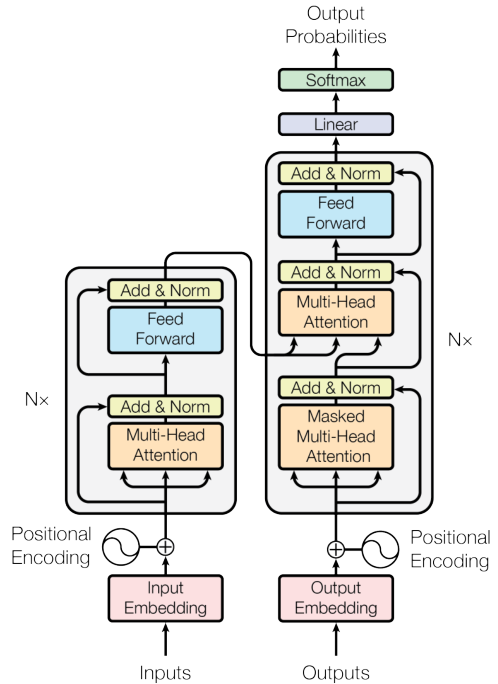
\includegraphics[scale=0.4]{abb/transformer-figure.png}
  \end{center}
  \caption{entommen aus "Attention Is All You Need"}
\end{figure}
\subsubsection{BERT}
Das BERT Modell ist wieder ein großer Meilenstein im NLP Bereich und
kann als einer der ersten Large Language Models betrachtet werden.
Das Modell verbessert die Transformer Architektur indem es die
Embeddings der Token verbessert, zwei neue Trainingsaufgaben einführt
und aussschließlich Encoder verwendet.
\begin{figure}[H]
  \begin{center}
    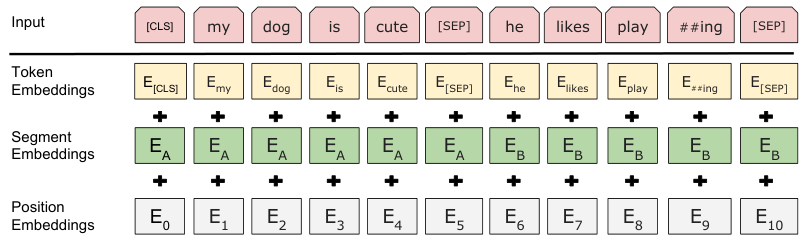
\includegraphics[scale=0.5]{abb/BERT-Tokens.png}
  \end{center}
  \caption{Token Embedding Prozess entnommen aus dem BERT Paper.}
\end{figure}
In Abbildung 2.8 ist der Token Embedding Prozess abgebildet, der
im folgenden näher beschrieben wird. Zunächst muss erläutert 
werden was ein  Token ist. Ein {\bf Token} ist in unsere Fall ein Wort,
aber generell ist ein Token, eine kleinere Zeichenkette die aus
einen Text gewonnen wird und einer Bedeutung zugewiesen wird
oder in eine Zahl umgewandelt wird um die weiterverarbeitung
zu vereinfachen.\\
Das BERT Modell addiert drei unterschiedlich informationen
in Vektorform auf, um noch bessere Token Embeddings zu
generieren. BERT benutzt WordPiece %(Quelle)
um die Token Embeddings zu bekommen, auf diesen wird
nun noch ein Segement Embedding und schließlich Position
Embedding darauf addiert. {\bf Segment Embedding} kodiert
die Information welche Tokens strukturell zusammen gehören
(Bspw. ein Satz). Das {\bf Position Embedding} kodiert
die sequentielle Position im Input.\\
Das wichtigste Puzzleteil sind die zwei unterschiedlichen
Trainingsaufgaben. Während der Transformer strikt die
Token von links nach rechts vorhersagt, wird BERT darauf
trainiert Wörter die auf beliebiger Position fehlen 
vorherzusagen, deswegen hat das Modell zugriff auf
den Kontext der sich links und recht von dem zu verhersagenden
Token befindet. Die Autoren bennenen diese Trainingsform
{\bf Masked Language Modeling}, es werden $15\%$ der Input
Tokens durch, entweder das \verb|[Mask]| Token oder mit einen
zufälligen anderen Token ersetzt. Dabei bleiben 
$10\%$ der Tokens die maskiert werden sollten doch gleicht,
weitere $10\%$ davon werden durch ein zufälligen anderen Token
ersetzt und die restlichen $80\%$ davon werden durch
das \verb|[Mask]| Token ersetzt. Die zweite Traininsaufgabe
ist {\bf Next Sentence Prediction} (NSP), bei dieser Aufgabe
muss das BERT Modell bei der Eingabe von zwei Sätzen entscheiden,
ob diese sequentiell nacheinander kommen oder nicht. Dabei sind
$50\%$ der Daten, zwei Sätze die nacheinander kommen und
bei den anderen $50\%$ wird zu einen gegebenen Satz aus den gesamten
Daten ein zufälliger nicht sequentieller Satz gewählt. Um eine vorhersage zu
treffen,
ob die Sätze nacheinander kommen oder nicht wird das konstante \verb|[cls]|
Token Embedding verwendet, welches immer an erster stelle steht.
Der erster Outputvektor korrespondiert dann mit dem \verb|[cls]| Token und
wird verwendet um den Output \verb|isNext| oder \verb|notNext| zu produzieren.\\ 
Nachdem Training erhält man aus BERT die Outputvektoren welche genau gleich viele
sind wie der Inputvektoren, diese kann man dann mit wenig aufwand
weiter verwenden, um das Modell für bestimmte Probleme in NLP
anzupassen (engl. fine-tuning).

\subsubsection{Sentence Transformer}
Das Sentence-BERT (Reimers et al. 2019) Modell ist Stand der Technik,
im semantischen kodieren von natürlicher Sprache in einem Vektorraum.
Die Implementierung der Autoren ist unter den Namen Sentence-Transformer 
(\underline{LINK??})
bekannt und wird in dieser Arbeit verwendet. Die Motivation hinter Sentence-BERT
(SBERT) ist das effiziente semantische vergleichen von zwei Sätzen. Wenn man mit
BERT herausfinden will, wie semantisch ähnlich zwei gegebene Sätze sind, dann muss 
man beide als Input in das Modell eingeben. Dass heißt wenn man die Ähnlichkeit
von allen $n$ Sätzen jeweils zueinander haben will, gibt es $\frac{n(n-1)}{2}$
eingaben in das BERT Modell, die man tätigen müsste. Bei SBERT allerdings kann 
nun jeder Satz einzeln eigegeben werden, der resultierende Ouput ist dann 
ein semantischer Vektorraum, indem jeder Satz ein semantischen Vektor besitzt.
Um jetzt die semantische ähnlichkeit zwischen zwei Vektoren zu erhalten, müssen
beide Vektoren nur in eine zu wählende Metrik eingesetzt werden. In den Paper
wird die Kosinus-Ähnilichkeit verwendet: Sei $u,v \in \mathbb{R}^n$, dann setze
\[
  Kos(u,v) := cos(\phi) = \frac{u \cdot v}{\|u\|\|v\|} 
  = \frac
  {
    \sum_{i=1}^n u_iv_i
  }
  {
    \sqrt{\sum_{i=1}^n u_i^2} \sqrt{\sum_{i=1}^n v_i^2}
  }.
\]
Damit kann dann effizient die semantsiche Ähnlichkeit zwischen zwei Vektoren
berechnet werden. Die Modellarchitektur von SBERT wird als {\bf Siamese Neural Network }
bezeichnet, da scheinbar zwei unterschiedliche BERT Modelle verwendet werden
um beide Sätze in einen Vektor umzuwandeln, aber beide Modell teilen sich 
die Gewichte. 
\begin{figure}[H]
  \begin{center}
    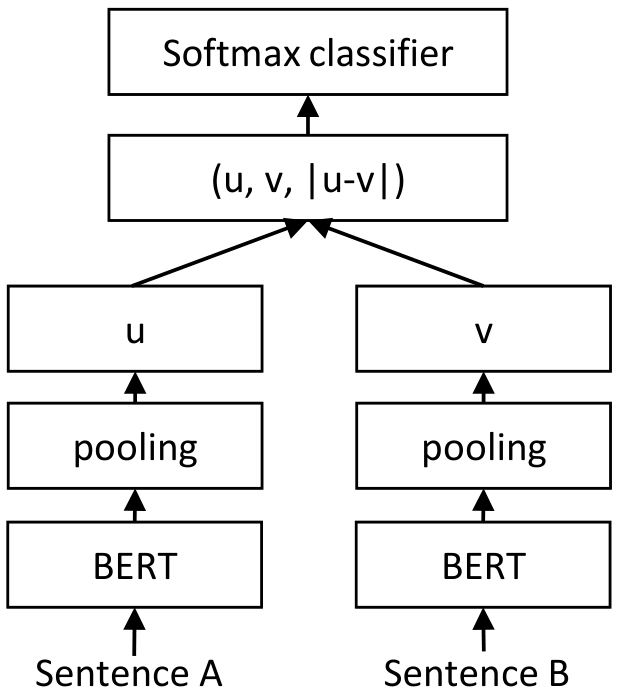
\includegraphics[scale=0.3]{abb/SBERT.png}
  \end{center}
  \caption{SBERT Architektur entnommen aus dem SBERT Paper.}
\end{figure}
In Abbildung 2.9 ist die SBERT Sieamese Neural Network Architektur abgebildet,
das heißt dass sich beide BERT Modelle die selben Geweicht teilen. Danach
geht der Output von BERT in ein pooling Modul. {\bf Pooling} ist das transformieren
von Output mit vielen Vektoren in eine geringere Anzahl von Vektoren oder 
Dimension. In unseren Fall werden die $n$ Output Vektoren von BERT in einen 
einzigen Output Vektor transformiert. Das in dem Paper verwendete
default pooling ist der Mittelwert, d.h. auf alle Ouputvektoren von BERT,
wird das arithmetische Mittel angewendet, daraus erhält man einen Vektor
mit den Mittelwerten der jeweiligen BERT Output Vektoren. Desweiteren wird
das BERT Modell noch einwenig, auf die spezielle aufgabe, zwei Vektoren
semantisch zu vergleichen, angepasst. Dafür wird der SNLI Datensatz verwendet,
dieser beinhaltet immer zwei sätze und eins von drei möglichen Label:
\verb|contradiction|, \verb|neutral|, und \verb|entailment|. Also muss SBERT
für zwei sätze vorhersagen ob sie sich inhaltlich wiedersrpechen, neutral
zueinander sind, oder der eine Satz eine Fortsetzung des anderen ist. Daraus
lernt das Modell ein semantisches verständis für Sätze zu erlangen. Beim Training
wird um die label Vorhersage zubekommen, wie in Abbilding 2.9 dargestellt,
die jeweiligen Vektoren und ihre Differenz konkatiniert. Anschließend werden
diese mit einen lernbaren Gewicht multipliziert, sodass ein Vektor mit 
drei Dimensionen herauskommt, dann wird der Softmax angewendet.
Die Position in dem Vektor mit dem höchsten Wert wird schließlich dem zugehörigen
Label zugeordnet. Mathematisch: \\Sei $W \in \mathbb{R}^{n\times 3}$
das lernbare Gewicht und $v \in \mathbb{R}^n$ Outputvektor von pooling, dann
\[
  o = \text{softmax}(Wv).
\]
Nachdem Training, bei der Inferenz wird der Vektor nachdem pooling als 
ouputvektor ausgeben.\\
SBERT liefert uns also ein Tool, um Sätze semantisch in einen Vektorraum
abzubilden, welches sich in späteren Kapitelen als sehr hilfreich herausstellt.
\subsection{Code-Llama}
Die Code-Llama famillie an Large Language Models, wurde von Meta AI im Jahre
2024 entwickelt. {\bf Large Language Models} sind Modelle, die auf einer
großen Menge von Daten trainiert wurden, welche sich darin auszeichnen,
natürliche Sprache verstehen sowie generieren zu können und deswegen in 
der Lage sind, eine Vielzahl von Aufhaben im NLP-Bereich zu lösen.
Meta AI Optimiert das vorangegangene Llama2 Modell, auf programmiersprachen 
spezifischen Aufgaben. Das LLama2 Model wird um zum resultierenden Code-llama
zu kommen, erneut auf einen neuen Datensatz trainiert. Dieser besteht aus
drei verschieden kategorien von Daten. Der größte Teil im Datensatz mit
$85\%$, ist der mit
Programmiersprachen spezifischen aufgaben, indem wird das Modell darauf 
trainiert fehlende Programmzeilen in einer vorgebenen Lücke zu füllen.
Dabei kann es sich um Befehle, aber auch um Kommentare handeln. Der zweit 
größte Teil im Datensatz mit $8\%$, besteht aus natürlicher Sprache in der 
es um programmcode geht. Dieser Teil beimhaltet diskussion über Programmcode
,sowie Fragen und Antworten welche sich auf Programmcode beziehen. Der kleinste
Teil im Datensatz mit $7\%$ besteht aus belibiger natürlicher Sprache, damit
das Modell seine alten fähigkeiten erhält. \\
Das LLama2 Modell ist eine Verbesserung des Llama1 Modells. Dieses wurde auf
neuren Daten Trainiert und verwendet einen $40\%$ größeren Datensatz.
Deweiteren wurde die {\bf context length} verdoppelt, welche die maximale
Anzahl der gleichzeitig zu verabeitende Token beschreibt. Außerdem gab es
eine veränderung in der Llama1 Transformer Architektur. In den Attention 
Modulen werden zwei Werte die normalerweise jedesmal wieder berechnet
werden geteilt, d.h. jedes Attention Modul hat Zugriff auf die gleichen
Werte. Das führt zu etwas schlechteren Ergebnissen, aber einer deutlichen
Leistungs steigerung.\\
Das Llama1 Modell wiederum besteht aus einer Decoder-Only Transformer
Architektur. Der {\bf Decoder-Only Transformer} besteht wie der Name es schon
vermuten lässt, nur aus Decoder Transformer Blöcken. Bei dieser Architektur
ist der anfängliche Input des Decoders, die Einabe des Nutzers. Auf diese
Eingabe wird dann immer wieder das neu generierte Token konkatiniert. Auf diese
weise wird die Eingabe nicht explizit von dem bereits generierten getrennt
sondern beides wird als bereits generierter Kontext verwendet. Das besondere
an Llama1 ist das es nur auf frei verfügbaren Daten trainiert wurde und 
dass das Modell Open Source ist. Der Datensatz besteht aus {\bf English 
Common Crawl [$67\%$]}, {\bf C4 [$15\%$]}, {\bf Github [$4.5\%$]},
{\bf Wikipedia [$4.5\%$]}, {\bf Gutenberg and Books3 [$4.5\%$]}, 
{\bf ArXiv [$2.5\%$]}, und {\bf Stack Exchange [$2\%$]}.\\
Code Llama ist Open-Source und schneidet unter allen öffentlich verfügbaren
Modellen am besten in multilinugal Benchmarks ab. Mit multilingual ist hier die
verwendung von mehreren Programmiersprachen gemeint. Diese 
Eigenschaften machen es sehr geignet für diese Arbeit.
\subsection{Code2Vec}
Cod2Vec ist eine im Jahre 2018 entwickelte Modellarchitektur, die Quellcode in
einen semantischen Vektor kodiert. Nach den vielen erfolgen in NLP, natürliche
Sprache in semantische Vektoren zu kodieren, ergab sich der natürliche wunsch
auch Quellcode in semantische Vektoren abzubilden. Mit diesen Vektoren kann
dann wieder viele verschiedene Aufgaben gelöst werden. Das motivierende Beispiel
im Code2Vec Paper ist dem Quellcode einer Funktion einen sinvollen Namen 
vorherzusagen. Im folgende wird die Architektur die in Abbilding 2.10 zusehen
ist erklärt. 
\begin{figure}[H]
  \begin{center}
    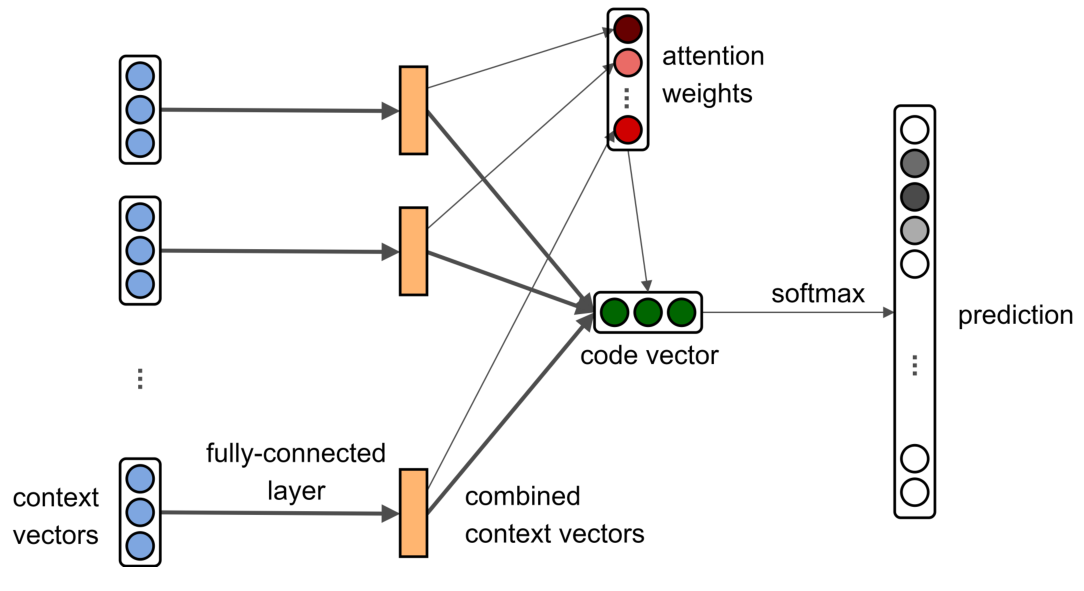
\includegraphics[scale=0.3]{abb/code2vec.png}
  \end{center}
  \caption{Code2Vec Architektur entnommen aus dem Code2Vec Paper}
\end{figure}
Die Autoren fanden heraus das eine geignete Darstellung von Quellcode
als ein mathematisches Objekt ein abstraketer Syntaxbaum ist. Dieser erhält 
die strukturellen zusammenhänge zwischen den Tokens und kann gut in einen
Vektor kodiert werden. Die Inputvektoren (context vectors) bestehen jeweils aus
einen Pfad im abstrakten Syntaxbaum, mit dem jeweilligen Starttoken und
Endtoken des Pfades. Danach folgt ein Hidden-Layer, mit \verb|tanh| als
Aktivierungsfunktion. Der finale Vektor (code vector) berechnet sich einfach
als linear kombination aus den Ouputvektoren und den attention weights. Sei
$h_1, \dots, h_n \in \mathbb{R}^d$ die Outputvektoren von dem Hidden-Layer
und $\alpha \in \mathbb{R}^n$ der attention weights Vektor.
\[
  \verb| code vector | v = \sum_{i = 1}^n \alpha_i \cdot h_i
\]
Mit dem \verb|code vector| kann dann das gewünschte Label vorhergesagt werden.
Das Modell kann demnach darauf trainiert werden ein bestimmtes Label 
vorherzusagen, welches zu einen Quellcode, also einer reihe an 
\verb |context vector| zugerodnet wird. Nachdem Training kann es dann auch 
Label für Quellcode vorhersagen die es noch nie gesehen hat.\\
Die Trainingsart ist demnach Überwachteslernen, was eine aufbereitung der 
Daten benötigt. Das Modell kann deswegen auch nur Label vorhersagen in der
Inferenz, die es vorher im Training gesehen hat.
\subsection{t-SNE}
{\bf t}-Distributed {\bf S}tochastic {\bf N}eigbor {\bf E}mbedding ({\bf t-SNE})
ist ein Algorithmus, welcher zum visualisieren von hochdimensionalen Daten 
eingesetzt wird. Um das zu ermöglichen reduziert t-SNE die Dimension von 
$n \in \mathbb{N}$ zu einer niedrigeren Dimension wie zwei oder drei, inder
der Mensch die Datenpunkte leicht interpretieren kann, ohne die 
Nachbarschaftsverhältnisse der Datenpunkte in mitleidenschaft zu ziehen.\\
Im folgende wird der Algorithmus skizziert und danach wird aufgezeigt was bei 
der effektiven verwendung von t-SNE zu beachten ist. Die hochdimensionalen 
Datenpunkte werden mit $\mathbf{H}$ und die niedrigdimensionale Datenpukte mit
$\mathbf{N}$ bezeichnet. Der erste schritt des Algorithmuses ist es 
jedem Datenpunktpaar im Datensatz $\mathbf{H}$ ein Ähnlichkeitsscore zu zuweisen.
Dieser wird berechnet indem man zuerst die euklidische Distanz von jeden Datenpaar
berechnet und dann das Ergebnis in eine Wahrscheinlichkeitsverteilung eingibt,
dadurch wird der Wert unter anderen Normalisiert. Das Ergebis ist dann eine 
Tabelle mit einen Ähnlichkeitsscore für jedes Datenpaar in $\mathbf{H}$. Als
nächstes werden die Datenpunkte zufällig in der niedrigen Dimension 
$\mathbf{N}$ angeordnet. Die nachfolgenden zwei schritte werden $T\in \mathbb{N}$
mal wiederholt, wobei $T$ ein Parameter ist der wählbar ist.
\begin{enumerate}
  \item Berechne Ähnlichkeitsscore von $\mathbf{N}$, diesmal wird aber die
      studentische t-Verteilung als wahrscheinlichkeitsverteilung genommen. 
  \item Verschiebe die Datenpunkte von $\mathbf{N}$ um ein kleinen Wert in
    die Richtung, die den Unterschied der Ähnlichkeitsscores von $\mathbf{H}$
    und $\mathbf{N}$ minimiert.
\end{enumerate}
Nach $T$ wiederholung ist der Ähnlichkeitsscore von $\mathbf{N}$ und $\mathbf{H}$
nahe bei einander, d.h. die Nachbarschaftsverhältniss von $\mathbf{N}$ und 
$\mathbf{H}$ sind nun ähnlich.\\
Mitarbeiter von Google haben untersucht, wie man t-SNE sinvoll anwendet und
welche schlüsse man aus der visualisierung ziehen kann. Sie fanden heraus,
dass die wahl der Parameter für das Ergebnis eine wichtige Rolle spielen.
Die wichtigsten Parameter sind die Iterationen $T\in \mathbb{N}$ und die
Perplexity $P \in \mathbb{N}$. Die {\bf Perplexity} kann intuitiv als schätzung 
für die Anzahl an nahen Nachbarn die jeder Datenpunt hat gesehen werden.
Eine geignete Iteration $T$ kann relative einfach durch ausprobieren 
herausgefunden werden: Falls sich die Datenwolke bei erhöhung von $T$
nicht mehr wirklich verändert, ist die Anzahl der Iteration $T$ gefunden
worden. Eine geeignete Perplexity zu finden ist schwieriger, da wir die
hochdimensionalen Nachbarschaftsbeziehungen meistens nicht kennen. Die Autoren
des t-SNE Paper empfehlen eine Perplexity $P \in \{5,6, \dots, 50\}$. Außerhalb
dieses Bereiches können verschieden ungewollte Phänomene auftreten. Bei $P=2$
haben die Google Mitarbeiter herausgefunden das t-SNE bei einer zufällig generierten
Datenwolke, fälschlicher weise kleine Gruppierungen (Cluster) bildet. Falls
$P$ größer ist als die Anzahl der Datenpunkte, ist das Ergebnis überhaupt nicht
interpretierbar. Es ist also immer Sinvoll, mehere Werte für $P$ aus zuprobieren,
um sicher zu gehen das t-SNE keine falschen Nachbarschaftsbeziehungen darstellt.
Die Mitarbeiter von Google fanden ausßerdem heraus, dass sowie die Information 
der Breite eines Clusters, als auch der Abstände von einen Cluster zu einen anderen 
durch t-SNE komplett verloren gehen. Es kann also nach betrachten der
t-SNE Ausgabe keine Aussage über den Durchmesser eines Clusters, die Position
des Cluster und die Lagebeziehungen zwischen Clustern getroffen werden. \\
Der t-SNE Algorithums ist ein wichtiges Tool um qualitative Aussagen über 
Daten zu treffen. Allerdings sollten immer mehrere Parameter ausprobiert werden.
Es kann nur eine Aussage über die existenz von Cluster getroffen werden und 
nicht über ihre geometrischen gegebenheiten. Wenn diese Rahmenbedingungen 
beachtet werden ist t-SNE ein sehr mächtiges visualisierung Tool um eine 
intuition von der Anordnung der Datenpunkte zu erhalten.
% effective use paper: 
% https://distill.pub/2016/misread-tsne/?_ga=2.135835192.888864733.1531353600-1779571267.1531353600
%pgf plots

%\subsection{Stand der Technik} in Introduction
% Self supervised learning (JTrans, PalmTree)
% Same Source policy (Safe)
%  Clap
\section{Methodik}
\subsection{Datensatz}
Im Maschinellen lernen hat der Datensatz bzw. die Trainingsdaten den
größten Einfluss auf die güte des Modells.
% Warum ist die Auswahl des Datensatzes wichtig
% Warum Glibc? 
% Gleicher Standard mit gleicher Semantik unterschiedlich Implementierung
\subsection{Datenpipeline}
Die große praktische Arbeit der Bachelorarbeit war es, eine große Menge
von Daten in verschiedensten Darstellungen immer wieder umzuwandeln. Dabei 
wurde jeder Zwischenschritt gespeichert, damit nicht jede Darstellung immer
wieder generiert werden muss. Im folgenden wird die generelle Architektur 
wie Daten verabeitet werden vorgestellt (engl. Pipeline), um ein Überblick
über den praktischen Teil dieser Arbeit zu geben.
\begin{figure}[H]
  \begin{center}
    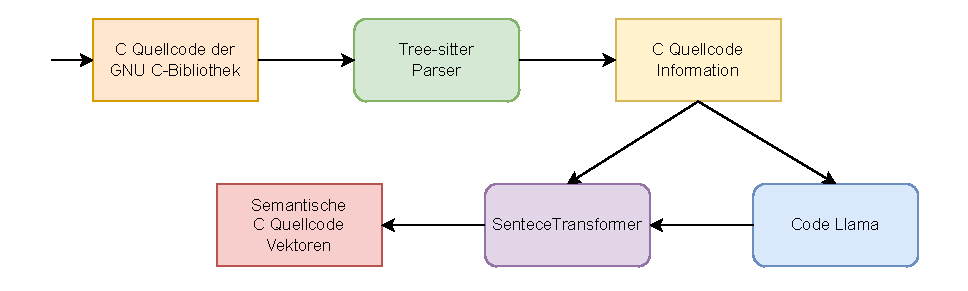
\includegraphics[scale=0.8]{abb/data-pipeline.pdf}
  \end{center}
  \caption{Datenpipeline}
\end{figure}
In der Abbildung 3.1 ist die Datenpipeline dargestellt, dabei sind Vierecke 
mit runden Ecken Tools die Daten in eine andere Darstellung umwandeln und
Vierecke mit spitzen Ecken repräsentieren Darstellungen von Daten. Die erste
Darstellung sind die Rohdaten, das entspricht den unverarbeiteten C Quellcode
aus der GNU Standard C Bibliothek. Nun brauche wir aber nicht alle Teile des
Quellcode sondern nur bestimmeteile, zum Beispiel arbeiten wir nur mit Funktionen
d.h. alle Datenstrukturen die in dem Quellcode definiert werden, wollen wir
aus dem Quellcode entfernen. Die Zerlegung und Umwandlung des Inputs 
in sinvolle Teile wird parsing genannt. In dieser Arbeit wurde {\bf Tree-sitter}
als Parser verwendet, welcher alle populären Programmiersprachen in Syntaxbäume
umwandeln kann. Ursprünglich wurde Tree-sitter für den Texteditor Atom entwickelt
und wird heute noch in vielen Texteditoren für bspw. Syntaxhighliting verwendet.
Generell kann Tree-sitter jedoch für alles das Quellcode verarbeiten will 
verwendet werden. Aus dem Syntaxbaum kann dann jeglich gewünschte Information 
entnommen werden. Diese Quellinformationen werden dann estmal zwischen gespeichert,
damit von nun an, die verabeitung hier angesetzt werden kann. Die Quellinforamtionen
beziehen sich immer auf eine Funktion, also ist das Format eine Tabelle die
für jede Funktion in den Rohdaten die gewünschten Quellinforamtionen enthält.
Danach gibt es eine Abzweigung, entweder werden die Quellinformationen Code Llama
nochmal erklärt und dann in den SentenceTransformer gegeben oder die 
Quellinformation wird direkt in den SentenceTransformer gegeben. Schließlich 
erhält man wieder eine Tabelle die gespeichert wird, die für jede Funktion
das zugewisene Semantische Embedding enthält. Bei dieser Architektur kann
mühelos jedes Tool ausgewechselt werden solange die Ausgabeformate eingehalten
werden.
% Treesitter erklären
% Source Code information in json datei speichern
% Dann Source code information in Vektor umwandeln
% Modularität -> Vorteile dieses Designs 
\subsection{Stabilität von SentenceTransformer}
In dem vorherigen unterkapitel haben wir gesehen das der finale schritt 
für alle Daten der SentenceTransformer ist, deswegen ist er das Herzstück
der Datenpipeline. In dieser Arbeit sollen verschiedene semantische 
beschreibungen des Quellcodes in natürlicher Sprache verglichen werden.
Um ein hier sinvoll zu messen müssen , wie bei einem physikilischen Experiment,
alle anderen Elemente in der Datenpipeline konstante Ergebnisse liefern und 
nicht schwanken. Aus diesen Gründen wird im folgenden Untersucht, wie stabil
sich der SentenceTransformer bei selber Eingabe verhält. Im optimafall sollte
der SentenceTransfomer bei selben Input selbes Ergebnis liefern. 


% Label Prozess sollte stabil sein bzw. deterministisch, sonst
% kann keine aussage über die Güte der Labels getätig werden
% Tabelle mit Ergebnissen der standardabweichungen

\
\section{Funktionskommentare}
\subsection{Motivation}
Bevor ein Programm kompelliert wird und nur noch die nötigsten Informationen
für den Computer bestehen bleiben, gibt es eine Menge an Informationen die 
die Semantik der Funktion in natürlicher Sprache beschreiben. Eine offensichtliche
Quellcodeinformation die im optimalfall die Semantik der Funktion in natürlicher
Sprache beschreibt ist der Kommentar. Ein gelungener Kommentar für eine Funktion
beschreibt präzise die kernfunktion der Prozedur, d.h. der Input, den Output
und wie diese umwandlung erfolgt. Dieser könnte man dann mit dem 
SentenceTransformer in einen Semantischen Vektoraum abbilden, was in einen
Semantischen Quellcode Vektor resultiert.
% Warum könnten funktionskommentare dafür geignet sein die Semantik einer
% Funktion zu beschreiben
\subsection{Methodik} 
Das parsen der Kommentare wurde wie in dem Unterkapitel Datenpipeline erwähnt 
mit Tree-sitter realisiert. Dabei gab es zwei große Designentscheidungen zu treffen.
Zum einen welche Kommentare in einer Funktion berücksichtigt werden sollen und
zweitens was macht man mit Funktionen die eine leicht Variationen von einer
anderen Funktion sind und deswegen keine Kommentare besitzten. Ein gutes Beispiel
für das zweite Problem ist \verb|exit| und \verb|__run_exit_handlers|, wenn
\verb|exit| aufgerufen wir, ruft diese Funktion einfach 
\verb|__run_exit_handlers| mit speziellen Parametern auf. Dabei ist \verb|exit|
nicht kommentiert, aber \verb|__run_exit_handlers| ist kommentiert.\\
{\color{red} Bei der ersten Designentscheidung welche Kommentare ich berücksichtige,
habe ich mich ausschließlich für den Kommentar direkt über der Funktion 
entschieden, da die einzeiligen Kommentare in der Funktion meistens keinen
großen Semantischen Wert haben, sondern auf gefahren oder Designentscheidungen
 hinweisen. (Beleg maybe: A survey on Reasearh of code comment)} Für das zweite Problem habe ich mich für folgende Lösung entschieden.
Falls eine Funktion keinen Kommentar besitzt, dann werden die Kommentare von
allen Funktionen die in den Funktionskörper aufgerufen werden konkatiniert und
als eigenen Kommentar übernommen. Dardurch hat \verb|exit| dann einen Kommentar
und zwar exakt den selben wir \verb|__run_exit_handlers|.\\
Hierbei muss man aufpassen das der Prozess des parsens nicht zu speziell an
den vorliegenden Daten angepasst wird, sonst verliert er seine Allgemeingültigkeit.
Deswegen habe ich mich nicht auf weitere Optimierungen die ein wenig mehr Kommentare
erbrignen könnten eingelassen, sondern es bei den oben beschriebenen belassen.
% Probleme beim Parsen, wo sucht man nach Kommentaren?
% Keine einheitliche Konvention
% -> Unterschiedliche Code Base Unterschiedliche Kommentar Konventionen
\section{Code2Vec}
\subsection{Motivation} 
Das besondere an Code2Vec ist, dass es den Quellcode in eine abstrakten
Syntaxbaum kodiert. Damit nutzt Code2Vec alle Quellcodeinformationen die
in dem Quellcode vorhanden sind. Danach wird das Modell darauf trainiert
eine Eigenschaft in natürlicher Sprache über den Quellcode vorherzusagen.
Bei dieser herangehensweise wird also kein SentenceTransformer verwendent
sondern der Semantische Vektroraum wird durch Training des Code2Vec Modells
als Nebenprodukt erzeugt. Wie in den Paper wird auch hier Code2Vec
darauf trainiert Funktionsnamen vorherzusagen. Leider wurde das Code2Vec
Modell nur auf Java trainiert, deswegen gab es einige anpassungen die 
die angwendet werden mussten. Da das Code2Vec Modell
auf überwachtes Lernen basiert, muss der Datensatz vor dem Training
erstmal aus den ursprünlgichen Quellcode aufbereitet werden.
% Warum könnte code2vec semantisch gute Vektoren produzieren
\subsection{Adaption auf C}
Um das Cod2Vec Modell Trainineren zu können muss aus den rohen Funktionen
jeweils ein abstrakter Syntaxbaum und den Funktionsnamen extrahiert werden.
Glücklicherweise hat JetBrains ein Tool entwickelt namens astminer. Das Tool
{\bf astminer}  wurde von dem JetBrains Research Team entwickelt, 
um Quellcode in abstrakte Syntaxbäume zu kodieren, für maschinelles Lernen
Modelle.



% code2vec erklären
\subsection{Training}
% Ganzes engeneering und pain hinter code2vec
\section{Funktionsnamen}
\subsection{Motivation}
% Motivation warum es gute semantische Vektoren erzeugen konnte
\subsection{Methodik}
% Parsen
% Eigentlich einfach aber wenn man in Zukunft 
% Viele System nahe sprachen dazu nehmen will
% wie Rust, C, Zig, usw. 
% Ist es doch schwieriger
% -> Treesitter
\section{Coddelama-Erklärungen}
\subsection{Motivation}
%Warum LLM's gute Embeddings produzieren könnten.
%Wir erzeugen uns eine zusammenfassung vom code
% "optimale" Kommentare
\subsection{Codellama} 
% Was ist Codellama und warum benutzten wir es?
\subsection{Prompt Engeneering und Temperature}
% Von Chatbot zu relativ deterministischen Modell
% Ergebnisse der Standardabweichung mit Temperatur 0
\section{Ergebnisse}
\subsection{Evaluierung durch Experten}
\subsubsection{Methodik}
% Aufbau des Fragebogens und
% Stichproben Größe, vlt. Vorstellung der Experten
\subsubsection{Auswertung und Ergebnisse}
% Diskussion der Ergebnisse
% Folgerungen das CodeLlamma "gute" Embeddings produziert 
\subsection{Qualitative Evaluierung} 
% t-SNE Plots
% Vielleicht nochmal subsections mit Funktionsname, Funktionskommentare, 
% Funktionserklärung, und Code2Vec Vektoren
% Probleme des jeweiligen Ansatzes mit drei Vektoren
\subsection{Quantitative Evaluierung} 
% Formel um zwei Embedding spaces zu vergleichen
% Formel erklären und rechtfertigen
% Aus Umfrage rechtfertigen Codellama Summaries als gute
% embeddings zu verwenden
\section{Limitation}
\section{Diskussion}
%copy Evaluation
% Zusammenfassung der jeweiligen Resultate
% Funktionnamen -> Nicht geignet, da zu wenig informationen und abkürzungen
% Funktionskommentare -> Je nach Projekt geignet, aber nicht allgemeingültig
%     deswegen eher ungeignet
% Code2Vec -> Kommt nur knapp an mit benutzuten Daten an Names ran also nicht 
% geignet
\section{Fazit}
\section{Results: Comparing natural language supervised methods for creating Rich Binary Labels}
\begin{itemize}
  \item Stabilität von Sentence Transformer
  \item Kommentare von Funktionen um Embeddings zu generieren
  \item Funktionsnamen von Funktionen um Embeddings zu generieren
  \item Code2Vec um Embeddings zu generieren
  \item CodeLlama Erklärungen von Funktionen um Embeddings zu generieren
  \item Evaluierung durch tSNE-Plots
  \item Evaluierung durch Experten
  \item Evaluierung durch Formel
\end{itemize}
$ I_{k}: \mathbf{N} \times \mathbf{N} \times \mathbf{N}^{k} \to [0,1]$
\[ I_{k}(x,i,v) = \begin{cases*} 
      1 & , $\exists j \in \mathbf{N}: x = v_j \land i = j$  \\
      \frac{1}{2} & , $\exists j \in \mathbf{N}: x = v_j \land i \neq j$\\
      0   & , \text{otherwise}
                \end{cases*} \]
$E_k: \nat^k \times \nat^k \to [0,1]$
\[ E_k(u,v) = \frac{1}{G_k} \sum^{k}_{i=1} \frac{I_k(u_i,i,v_i)}{log_2(i+1)}\]
wo $G_k := \sum_{i=1}^{k} \frac{1}{log_2(i+1)}$.\\\\
$CMP_k: \mathbf{R}^{N\times l} \times \mathbf{R}^{N\times l} \times 
\{ \mathbf{R}^l \times \mathbf{R}^{N\times l} \to \mathbf{N}^k \} 
\times \{ \mathcal{P}([0,1]) \to [0,1] \} \to [0,1]$

\[ CMP_k(X,Y,f_k,agg) = agg(\{E_k(f_k(X_{i,j},X),f_k(Y_{i,j},Y)) | j \in \{1,2,3, \dots N\}\})\]


\section{Conclusion}


\section{Notes on form}
\subsection{Formatting} 
This LaTeX template uses the following formatting:
\begin{itemize}
\setlength{\itemsep}{0pt}
	\item font: Linux Libertine O (alternatively: Times New Roman)
	\item font size: 12 pt
	\item left and right margin: 3.5 cm, top and bottom margin: 3 cm
    \item align: left
	\item line spacing: one and a half (alternative: 15 pt line spacing with 12 pt font size)
\end{itemize}

\noindent
When implementing the specifications in Word, it is essential to define style sheets.

\subsection{Citation} 
\label{sec:cit}

The citation method follows the author-year system. Place reference is in the text, footnotes should only be used for explanations and comments. The following notes are taken from the \emph{language} bibliography template from \url{ron.artstein.org}:\newline

\noindent
The \emph{Language} style sheet makes a distinction between two kinds of in-text citations: citing a work and citing an author.
\begin{itemize}
\item Citing a work:
  \begin{itemize}
    \setlength{\itemsep}{0pt}
    \setlength{\parsep}{0pt}
  \item Two authors are joined by an ampersand (\&).
  \item More than two authors are abbreviated with \emph{et al.}
  \item No parentheses are placed around the year (though parentheses
    may contain the whole citation). 
  \end{itemize}
\item Citing an author:
  \begin{itemize}
    \setlength{\itemsep}{0pt}
    \setlength{\parsep}{0pt}
  \item Two authors are joined by \emph{and}.
  \item More than two authors are abbreviated with \emph{and colleagues}.
  \item The year is surrounded by parentheses (with page numbers, if
    present).
  \end{itemize} 
\end{itemize}
To provide for both kinds of citations, \verb+language.bst+ capitalizes on the fact that \verb+natbib+ citation commands come in
two flavors. In a typical style compatible with \verb+natbib+, ordinary commands such as \verb+\citet+ and \verb+\citep+ produce short
citations abbreviated with \emph{et al.}, whereas starred commands such as \verb+\citet*+ and \verb+\citep*+ produce a citation with a
full author list. Since \emph{Language} does not require citations with full authors, the style \verb+language.bst+ repurposes the starred commands to be used for citing the author. The following table shows how the \verb+natbib+ citation commands work with \verb+language.bst+.
\begin{center}
  \begin{tabular}{lll}
    \toprule
    Command & Two authors & More than two authors \\
    \midrule
    \verb+\citet+ & \citet{hale} & \citet{sprouse} \\
    \verb+\citet*+ & \citet*{hale} & \citet*{sprouse} \\
    \addlinespace
    \verb+\citep+ & \citep{hale} & \citep{sprouse} \\
    \verb+\citep*+ & \citep*{hale} & \citep*{sprouse} \\
    \addlinespace
    \verb+\citealt+ & \citealt{hale} & \citealt{sprouse} \\
    \verb+\citealt*+ & \citealt*{hale} & \citealt*{sprouse} \\
    \addlinespace
    \verb+\citealp+ & \citealp{hale} & \citealp{sprouse} \\
    \verb+\citealp*+ & \citealp*{hale} & \citealp*{sprouse} \\
    \addlinespace
    \verb+\citeauthor+ & \citeauthor{hale} & \citeauthor{sprouse} \\
    \verb+\citeauthor*+ & \citeauthor*{hale} & \citeauthor*{sprouse} \\
    \verb+\citefullauthor+ & \citefullauthor{hale} & \citefullauthor{sprouse} \\
    \bottomrule
  \end{tabular}
\end{center}
Authors of \emph{Language} articles would typically use \verb+\citet*+, \verb+\citep+, \verb+\citealt+ and \verb+\citeauthor*+, though they
could use any of the above commands. There is no command for giving a full list of authors.

\section*{Bibliography}
The bibliography of this template includes the references of the \emph{language} stylesheet as a sample bibliography.

\pagebreak

\section{General Addenda}

If there are several additions you want to add, but they do not fit into the thesis itself, they belong here.

\subsection{Detailed Addition}

Even sections are possible, but usually only used for several elements in, e.g.\ tables, images, etc.

\section{Figures}
\subsection{Example 1}
\subsection{Example 2}


\pagebreak

\microtypesetup{protrusion=false}
\listoffigures{}
\listoftables{}
\microtypesetup{protrusion=true}

\clearpage
\printglossaries

\pagebreak

\addcontentsline{toc}{section}{Literatur}
\pagestyle{fancy}

\bibliographystyle{language-dt} %using language.bst
\bibliography{bibliography} %bib-filename

\nocite{*} %List all bib-entries

\end{document}
